% ==============================================================================
% SECTION 5.2: STYLIZED FACTS OF PERIPHERAL ACCUMULATION, DISTRIBUTION, AND EXTERNAL CONSTRAINTS
% ==============================================================================

\subsubsection{Structural Constraints of Peripheral Transition: An Accounting Anchor}
\label{sec:stylized_material_bounds}

The political mobilization and redistributive policies analyzed in Section~\ref{sec:historical_background} unfolded within external material constraints. The Chilean economy relied on imported machinery, intermediate spare parts, and foreign trade credits to sustain domestic employment and basic wage-goods production. Mainstream accounts \citep{DornbuschEdwards1990,Edwards2024} attribute the subsequent macroeconomic crisis to fiscal deficits and unconstrained money creation that depleted reserves and triggered inflation. In contrast, structuralist and dependency traditions \citep{Stallings1978,DeVylder1976} emphasize balance-of-payments vulnerability, intermediate import dependency, and external credit restrictions. Comparing these perspectives requires establishing the descriptive sequence between external balance-sheet deterioration, domestic inflation, and monetary expansion.

In a subordinate open economy without reserve-currency status, convertible international reserves constrain the ability of the central bank to settle external obligations, finance intermediate imports, and maintain exchange parity. To track this external balance-sheet position, I define the Central Bank Solvency Ratio relative to Base Money:
\begin{equation}
    \text{SolvR}^{H}_t \equiv \frac{e_t \cdot IR_t}{H_t \cdot 1000},
    \label{eq:solvency_ratio_base_def}
\end{equation}
where $e_t$ is the official exchange rate (standardized in pesos per USD in the Central Bank database), $IR_t$ represents gross international reserves in USD millions from the IMF (yielding a numerator $e_t \cdot IR_t$ in millions of pesos), and $H_t$ denotes domestic base money liabilities recorded in thousands of millions of pesos (billions, \emph{miles de millones de pesos}), scaled by $1{,}000$ to express liabilities in millions of pesos and ensure dimensional consistency. As foreign reserves fell and external credit lines contracted, reserve coverage of the domestic monetary base declined. The descriptive sequence therefore raises the empirical question of whether domestic money growth preceded inflation as an autonomous driver or responded to emerging external bottlenecks and domestic cost pressures.

\subsubsection{Long-Span Balance of Payments Accounting: Reserve Accumulation and the 1971 Capital-Flow Reversal (1958--1975)}
\label{sec:stylized_bop_accounting}

In standard national accounting, the annual change in official Central Bank international reserves ($\Delta IR_t$) satisfies the identity:
\begin{equation}
    \Delta IR_t \equiv CA_t + KA_t + EO_t + SDR_t
    \label{eq:bop_reserves_identity}
\end{equation}
where $CA_t$ is the current account balance, $KA_t$ denotes net capital inflows, $EO_t$ represents net errors and omissions, and $SDR_t$ denotes allocations of IMF Special Drawing Rights. Net errors and omissions represent an accounting residual that, in peripheral contexts confronting trade and exchange controls, is consistent with unrecorded capital flight and trade misinvoicing \citep{Stallings1978}. Two distinct reserve concepts must be separated throughout this analysis: gross international reserves ($IR_t$), which record total foreign exchange assets held by the monetary authority, and net international reserves ($IR^{\text{net}}_t$), which subtract short-term foreign liabilities from gross holdings.

\begin{landscape}
\begin{table}[!htbp]
\centering
\scriptsize
\caption{Long-Span Balance of Payments Accounting and International Reserves Dynamics (Chile, 1958--1975): Official BCCh Cash Flows vs. WBOP Global Accrual Accounts}
\label{tab:bop_reserves_accounting}
\renewcommand{\arraystretch}{1.15}
\setlength{\tabcolsep}{3.0pt}
\resizebox{\linewidth}{!}{%
\begin{tabular}{lrrrrrrrrrrrrrrrrrr}
\toprule
& \textbf{Ib\'a\~nez} & \multicolumn{6}{c}{\textbf{Jorge Alessandri (1959--1964)}} & \multicolumn{6}{c}{\textbf{Eduardo Frei Montalva (1965--1970)}} & \multicolumn{3}{c}{\textbf{Unidad Popular (1971--1973)}} & \multicolumn{2}{c}{\textbf{Junta (1974--75)}} \\
\cmidrule(lr){2-2} \cmidrule(lr){3-8} \cmidrule(lr){9-14} \cmidrule(lr){15-17} \cmidrule(lr){18-19}
\textbf{Metric / USD Millions} & \textbf{1958} & \textbf{1959} & \textbf{1960} & \textbf{1961} & \textbf{1962} & \textbf{1963} & \textbf{1964} & \textbf{1965} & \textbf{1966} & \textbf{1967} & \textbf{1968} & \textbf{1969} & \textbf{1970} & \textbf{1971} & \textbf{1972} & \textbf{1973} & \textbf{1974} & \textbf{1975} \\
\midrule
\multicolumn{19}{l}{\textbf{A. Official Cash-Basis Balance of Payments (Central Bank of Chile / Stallings 1978, USD Millions)}} \\[0.2em]
Current Account ($CA$) & --- & $-24.8$ & $-148.1$ & $-241.1$ & $-181.9$ & $-157.8$ & $-131.6$ & $-56.6$ & $-82.2$ & $-127.4$ & $-135.3$ & $-5.6$ & $-102.9$ & \textbf{$-205.5$} & \textbf{$-404.8$} & $-294.6$ & $-210.8$ & $-491.3$ \\
Capital Account ($KA$) & --- & 20.8 & 76.3 & 187.6 & 133.2 & 107.6 & 152.1 & 65.8 & 168.0 & 125.5 & 294.6 & 222.5 & 267.5 & \textbf{$-26.5$} & 327.4 & 242.3 & 228.0 & 298.7 \\
Net Errors \& Omissions ($EO$) & --- & 28.6 & 43.4 & $-55.1$ & $-0.3$ & 22.0 & 2.9 & 37.5 & 33.8 & $-21.5$ & $-41.4$ & $-42.4$ & $-72.9$ & $-84.5$ & \textbf{$-171.6$} & $-60.0$ & $-62.1$ & $-92.4$ \\
SDR Allocations ($SDR$) & 0.0 & 0.0 & 0.0 & 0.0 & 0.0 & 0.0 & 0.0 & 0.0 & 0.0 & 0.0 & 0.0 & 0.0 & 21.8 & 16.7 & 18.2 & 0.0 & 0.0 & 0.0 \\
\midrule
Net Reserve Change ($\Delta IR$) & --- & \textbf{24.6} & \textbf{$-28.4$} & \textbf{$-108.6$} & \textbf{$-49.0$} & \textbf{$-28.2$} & \textbf{23.4} & \textbf{46.7} & \textbf{119.6} & \textbf{$-23.4$} & \textbf{117.9} & \textbf{174.5} & \textbf{113.5} & \textbf{$-299.8$} & \textbf{$-230.8$} & \textbf{$-112.3$} & \textbf{$-44.9$} & \textbf{$-285.0$} \\
Net International Reserves ($IR^{\text{net}}_t$) & 29.6 & 105.4 & 72.8 & $-5.2$ & 15.4 & $-24.3$ & \textbf{$-16.5$} & 35.2 & 77.4 & 54.3 & 125.4 & 285.2 & \textbf{393.5} & 162.7 & \textbf{75.8} & 167.4 & 94.0 & \textbf{$-129.2$} \\
\midrule
\multicolumn{19}{l}{\textbf{B. Capital Account Reversal, External Drainage, and Cumulative Flows}} \\[0.2em]
Net External Drain ($CA+KA+EO$) & --- & $+24.6$ & $-28.4$ & $-108.6$ & $-49.0$ & $-28.2$ & $+23.4$ & $+46.7$ & $+119.6$ & $-23.4$ & $+117.9$ & $+174.5$ & $+91.7$ & \textbf{$-316.5$} & \textbf{$-249.0$} & $-112.3$ & $-44.9$ & $-285.0$ \\
Drain Share of $IR_{t-1}$ & --- & --- & --- & --- & --- & --- & --- & --- & --- & --- & --- & --- & --- & \textbf{80.4\%} & \textbf{153.0\%} & 148.2\% & 26.8\% & 303.2\% \\
Cumulative $\sum KA$ & --- & \multicolumn{6}{c}{$+\$677.6\text{M}$ (Alessandri Total)} & \multicolumn{6}{c}{\textbf{$+\$1,143.9\text{M}$} (Frei Montalva Total)} & \multicolumn{3}{c}{$+\$543.2\text{M}$ (UP Total)} & \multicolumn{2}{c}{$+\$526.7\text{M}$} \\
Cumulative $\sum CA$ & --- & \multicolumn{6}{c}{$-\$885.3\text{M}$ (Alessandri Total)} & \multicolumn{6}{c}{\textbf{$-\$510.0\text{M}$} (Frei Montalva Total)} & \multicolumn{3}{c}{$-\$904.9\text{M}$ (UP Total)} & \multicolumn{2}{c}{$-\$702.1\text{M}$} \\
\midrule
\multicolumn{19}{l}{\textbf{C. Global Accrual Balance of Payments (WBOP, \citealt{NievasPiketty2025})}} \\[0.2em]
WBOP Current Account (USD M) & $-271.8$ & $-189.5$ & $-155.3$ & $-265.4$ & $-194.4$ & $-308.2$ & $-212.8$ & $-103.4$ & $-179.4$ & $-135.9$ & $-70.9$ & $+61.8$ & $-147.7$ & \textbf{$-421.6$} & \textbf{$-550.8$} & $-618.1$ & $-105.5$ & \textbf{$-470.6$} \\
WBOP Current Account (\% GDP) & $-7.74\%$ & $-5.00\%$ & $-3.40\%$ & $-5.19\%$ & $-3.26\%$ & $-5.21\%$ & $-3.37\%$ & $-1.60\%$ & $-2.37\%$ & $-1.82\%$ & $-0.93\%$ & $+0.70\%$ & $-1.53\%$ & \textbf{$-3.64\%$} & \textbf{$-4.40\%$} & $-3.47\%$ & $-0.61\%$ & \textbf{$-5.85\%$} \\
Net Foreign Wealth / IIP (\% GDP)& $-67.0\%$ & $-69.3\%$ & $-61.7\%$ & $-58.1\%$ & $-54.3\%$ & $-57.9\%$ & $-59.2\%$ & $-61.1\%$ & $-53.5\%$ & $-56.7\%$ & $-57.4\%$ & $-50.2\%$ & $-54.6\%$ & $-47.7\%$ & $-49.4\%$ & $-33.6\%$ & $-46.4\%$ & \textbf{$-100.6\%$} \\
\bottomrule
\end{tabular}%
}
\vspace{0.3em}
\begin{minipage}{\linewidth}
\scriptsize
\textbf{Sources and Notes:} Official cash-basis Balance of Payments flows (1960--1975), Net Errors and Omissions, and SDR allocations sourced from the Banco Central de Chile (BCCh) REST API and Base de Datos Estad\'{\i}sticos (BDE), complemented by historical balance-of-payments ledgers. 1958--1959 cash entries sourced directly from \citet[Table~7.4, p.~178]{Stallings1978}, citing contemporary BCCh records. Net international reserves ($IR^{\text{net}}_t$) record liquid foreign exchange assets net of short-term central bank foreign liabilities, compiled from BCCh historical ledgers and \citet{Stallings1978}, accounting for negative net balances during the 1961--1964 exchange crises and 1975; gross foreign reserve assets from IMF International Financial Statistics remain positive in all years. Global accrual balance of payments series and Net International Investment Position (NIIP) sourced from the World Historical Balance of Payments Database \citep{NievasPiketty2025}. The balance-of-payments reserves identity holds exactly: $\Delta IR_t \equiv CA_t + KA_t + EO_t + SDR_t$. Discrepancies between cash and accrual accounts reflect distinct institutional accounting conventions: cash ledgers record physical foreign exchange settlements at the Central Bank window, whereas WBOP accrual accounts adhere to modern BPM6 standards, incorporating legally accrued but unpaid debt service (under the November 1971 debt moratorium), reinvested foreign mining profits, and global bilateral trade partner reconciliations. Both records confirm that in 1971, net external financing experienced a sharp contraction of $-\$294.0$ million ($KA = -\$26.5\text{M}$ vs. $+\$267.5\text{M}$ in 1970), equivalent in magnitude to $98.1\%$ of the calendar-year reserve drain ($\Delta IR = -\$299.8\text{M}$) before domestic fiscal emission accelerated in late 1972.
\end{minipage}
\end{table}
\end{landscape}


Table~\ref{tab:bop_reserves_accounting} reports the balance-of-payments ledger across eighteen years (1958--1975), spanning four developmental regimes in dialogue with \citet{Stallings1978} and the World Historical Balance of Payments database \citep{NievasPiketty2025}. The table presents both cash-basis and accrual-basis accounts. The official BCCh cash ledger \citep[Table~7.4, p.~178]{Stallings1978} records foreign currency settlements that crossed the Central Bank counter, capturing the liquid resources available to defend exchange parity and pay for imports. In contrast, the WBOP database \citep{NievasPiketty2025} reconstructs accounts under modern IMF BPM6 accrual standards, recording primary income debits and interest obligations as they legally accrued, including during the November 1971 debt moratorium.

The pre-1970 administrations established the external balance-sheet position inherited by the Unidad Popular. Under Jorge Alessandri (1958--1964), import liberalization and a fixed nominal exchange rate led to cumulative current account deficits of $-\$885.3$ million. By late 1961, liquid reserves were exhausted, forcing emergency import controls and an eventual currency float in October 1962 that generated an inflation spike; net reserves ended at $-\$16.5$ million in 1964. The Eduardo Frei Montalva administration (1964--1970) instituted a crawling peg and accumulated reserves through external borrowing supported by the Alliance for Progress \citep{FfrenchDavis1973}. Cumulative net foreign capital inflows across Frei's term totaled $+\$1,143.9$ million, while the cumulative sum of annual reserve changes was $+\$548.8$ million. Net capital inflows thus exceeded cumulative reserve accumulation by more than two to one ($208.4\%$), as net reserves rose from $-\$16.5$ million in 1964 to $\$393.5$ million at year-end 1970 (a net stock increase of $+\$410.0$ million; the difference from cumulative annual flows reflects valuation adjustments on non-dollar holdings and the netting of short-term foreign liabilities in the stock measure). The reserve buffer inherited by the UP was therefore anchored in foreign credit lines.

Following the constitutional nationalization of large-scale copper mining on July 11, 1971 (Law 17,450), external financing contracted sharply. Net capital inflows fell from $+\$267.5$ million in 1970 to $-\$26.5$ million in 1971 ($-\$49.9$ million in Stallings' autonomous capital series). In the audited 1958--1975 ledger, 1971 was the only calendar year with negative net capital inflows. This $-\$294.0$ million turnaround in the capital account was equivalent in magnitude to $98.1\%$ of the calendar-year reserve drain ($\Delta IR = -\$299.8$ million), reducing Central Bank liquidity before domestic price acceleration took hold in late 1972.

The reduction in external financing materialized through specific commercial channels. As documented by \citet{DeVylder1976} and \citet{PetrasMorley1975}, international commercial banks curtailed short-term trade credits to Chile from $\$220$ million to $\$35$ million, while the U.S. Export-Import Bank suspended project lending. Foreign suppliers increasingly required cash-in-advance confirmed letters of credit for food and fuel shipments, and replacement parts for imported mining machinery faced delays in foreign ports \citep{Stallings1978}. Net Errors and Omissions recorded negative residuals totaling $-\$389.0$ million across the UP triennium ($-\$72.9$M in 1970, $-\$84.5$M in 1971, and $-\$171.6$M in 1972). Following the September 4, 1970 election, the Santiago stock exchange declined by $48.6\%$ and commercial bank deposits contracted \citep{GirardiBowles2018}. The timing is consistent with capital flight and private asset liquidation beginning prior to the presidential inauguration. While the cash ledger shows positive capital inflows in 1972 ($+\$327.4$M), this reflected the capitalization of debt service following the November 1971 moratorium. On an accrual basis, the WBOP current account deficit widened to $-\$550.8$ million ($-4.40\%$ of GDP) in 1972 and $-\$618.1$ million ($-3.47\%$ of GDP) in 1973, while Central Bank net foreign reserves fell to $\$75.8$ million at year-end 1972.

Following the September 1973 coup, external commercial credits resumed ($KA = +\$228.0$M in 1974 and $+\$298.7$M in 1975), and bilateral debts were rescheduled through the Paris Club. When world copper prices fell in 1975, domestic expenditure compression reduced import volumes. External vulnerability remained visible in the 1975 accounts: the accrual current account deficit reached $-\$470.6$ million ($-5.85\%$ of GDP), net international reserves fell to $-\$129.2$ million, and manufacturing output contracted.

\subsubsection{Terms of Trade, Capacity to Import, and Real Structural Imbalance (1960--1980)}
\label{sec:stylized_terms_of_trade}

To evaluate external purchasing power and physical trade flows, Figures~\ref{fig:solvency_reserves}, \ref{fig:copper_gold}, and \ref{fig:import_capacity} trace the monthly trajectories of foreign reserves, commodity prices, and import capacity across 1960--1980 ($N=252$ continuous calendar months, yielding $N=250$ observations in the transformed econometric sample).

\begin{figure}[!htbp]
\centering
\caption{Central Bank Solvency Ratio ($\text{SolvR}^H$) and Gross International Reserves (1960--1980)}
\label{fig:solvency_reserves}
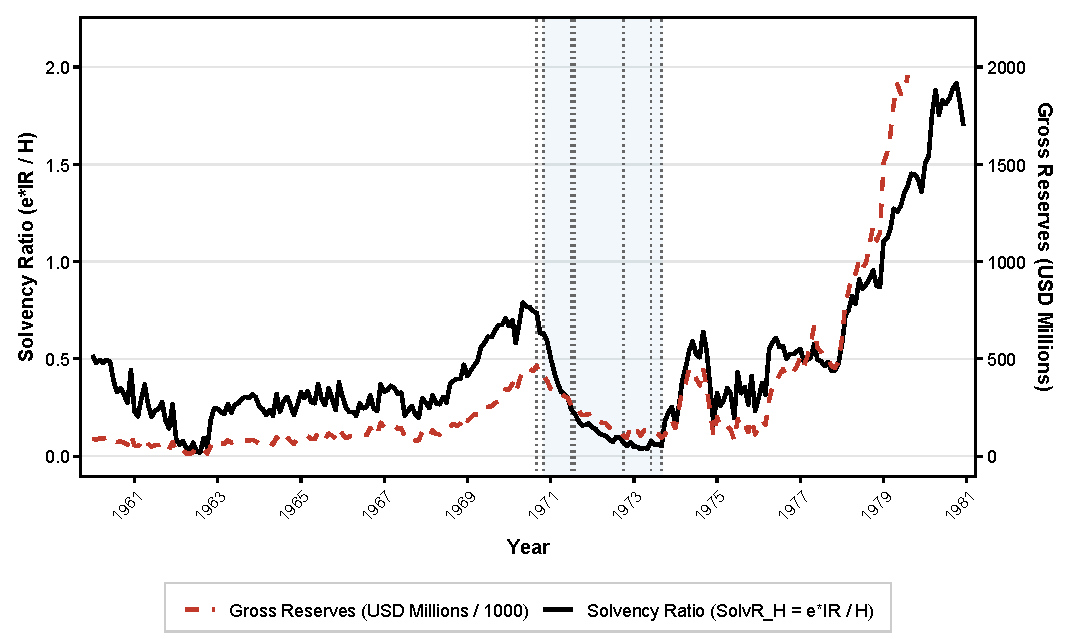
\includegraphics[width=0.88\textwidth]{figures/fig01a_solvency_reserves.pdf}
\begin{minipage}{0.95\textwidth}
\vspace{0.2cm}
\footnotesize
\textbf{Notes:} Monthly series tracking the Central Bank Solvency Ratio relative to Base Money ($\text{SolvR}^{H}_t \equiv \frac{e_t \cdot IR_t}{H_t \cdot 1000}$, left axis, solid black line) and IMF gross international reserves ($IR_t$ in USD millions, right axis, dashed red line). Base money ($H_t$) represents the Central Bank's direct domestic liability base from the archival ledger. Benchmark markers $\mathrm{I}$--$\mathrm{VII}$ defined in Table~\ref{tab:critical_junctures}. Shaded blue region designates the Unidad Popular government (November 1970 -- September 1973). Sourced from Central Bank of Chile REST API and IMF International Financial Statistics.
\end{minipage}
\end{figure}

\begin{figure}[!htbp]
\centering
\caption{World Copper Price and London Gold Price (1960--1980)}
\label{fig:copper_gold}
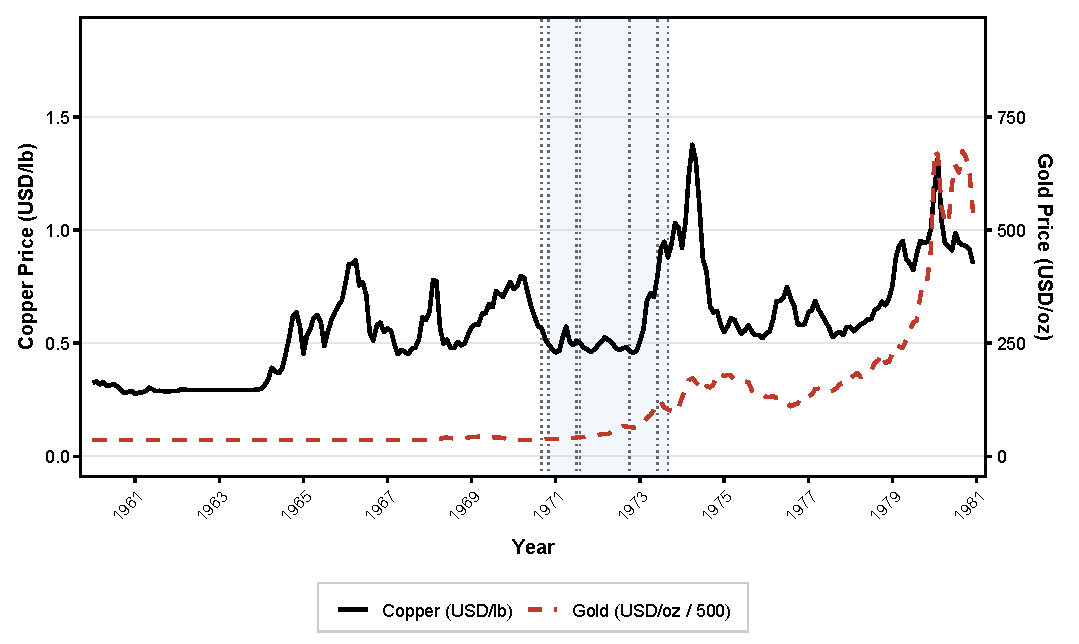
\includegraphics[width=0.88\textwidth]{figures/fig01b_copper_gold.pdf}
\begin{minipage}{0.95\textwidth}
\vspace{0.2cm}
\footnotesize
\textbf{Notes:} Monthly series tracking the London Metal Exchange copper cash price ($P^{\text{Cu}}$ in USD/lb, left axis, solid black line) and London Bullion Market Association gold price ($P^{\text{Gold}}$ in USD/oz / 500, right axis, dashed red line). Benchmark markers $\mathrm{I}$--$\mathrm{VII}$ defined in Table~\ref{tab:critical_junctures}. Shaded blue region designates the Unidad Popular government (November 1970 -- September 1973). Sourced from LME and LBMA via Central Bank of Chile REST API.
\end{minipage}
\end{figure}

The international terms of trade shifted unfavorably during the administration's first year (Figure~\ref{fig:copper_gold}). World copper export prices fell by $25\%$ during 1971, averaging $\$0.47$/lb compared to $\$0.64$/lb across 1969--1970, reducing export revenue during the initial domestic reactivation. Concurrently, the international monetary system absorbed the breakdown of the Bretton Woods architecture following the unilateral suspension of dollar-gold convertibility on August 15, 1971 (Benchmark $\mathrm{IV}$, \citealt{Zoeller2019,Vernengo2021}). The world gold price serves in this chapter as a proxy for the resulting international monetary turbulence and dollar inflation; gold prices rose past $\$100$/oz in 1973 and $\$200$/oz by 1978. In parallel, U.S. wholesale prices rose by $28.0\%$ between late 1970 and mid-1973 (Table~\ref{tab:marglin_monthly_grounding}), raising the foreign-currency price of imported goods.

\begin{figure}[!htbp]
\centering
\caption{Prebisch-ECLAC Real Capacity to Import and Effective Real Imports (1960--1980)}
\label{fig:import_capacity}
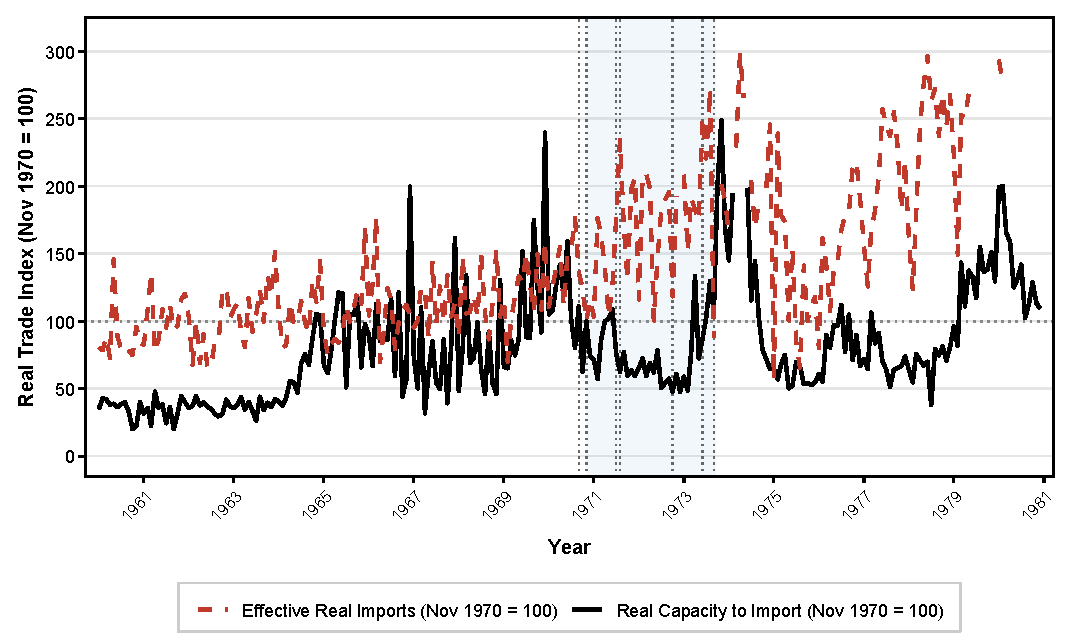
\includegraphics[width=0.88\textwidth]{figures/fig01f_import_capacity.pdf}
\begin{minipage}{0.95\textwidth}
\vspace{0.2cm}
\footnotesize
\textbf{Notes:} Monthly trajectory tracking the Prebisch-ECLAC Real Capacity to Import ($M^{\text{cap}}_t \equiv [\text{Exports}_t / \text{Exports}_{70:11}] \times [(P^{\text{Cu}}_t / P^{\text{Cu}}_{70:11}) / (P^{\text{US}}_{W,t} / P^{\text{US}}_{W,70:11})] \times 100$, solid black line) against Effective Real Imports ($M_t \equiv \text{Imports}_t / \text{Imports}_{70:11} \times 100$, dashed red line). Both series normalized to November 1970 = 100. Benchmark markers $\mathrm{I}$--$\mathrm{VII}$ defined in Table~\ref{tab:critical_junctures}. Shaded blue region designates the Unidad Popular government (1970--1973). Physical merchandise export and import volume series sourced from \citet{DiazBahamonde2023} historical database, compiled from \textit{Estad\'{\i}stica Chilena} and customs records (with April 1973 administrative registration drop interpolated); copper prices from LME via Central Bank of Chile REST API; U.S. wholesale prices from BLS.
\end{minipage}
\end{figure}

Figure~\ref{fig:import_capacity} compares external purchasing power with effective real import flows. When the world price of copper rose from $\$0.508$/lb in January 1973 to $\$0.948$/lb in August 1973, Central Bank gross international reserves remained low, fluctuating in a narrow range of $\$103$--$\$114$ million. The divergence reflected two offsetting movements. On the export side, transport disruptions and equipment shortages held back physical export volumes, muting the revenue gains from higher dollar copper prices. On the import side, effective real imports ($M_t$) expanded, reaching $234.5\%$ of the November 1970 baseline in August 1971 and $272.3\%$ in August 1973, driven by purchases of food, fuel, and intermediate goods.

Operationalizing the Prebisch-ECLAC Capacity to Import ($M^{\text{cap}}_t$), Figure~\ref{fig:import_capacity} documents that Chile's real export purchasing power fell from $100.0$ in November 1970 to $62.5$ in August 1971 and $47.7$ in October 1972 before rebounding in 1973. This generated a wide Real Structural Imbalance ($\Theta_t \equiv M_t / M^{\text{cap}}_t \times 100$), which reached $374.9\%$ in August 1971 and $346.4\%$ in December 1971 (Table~\ref{tab:marglin_monthly_grounding}). The descriptive sequence demonstrates that external balance-of-payments pressures and foreign-exchange scarcity were present well before the price acceleration of late 1972.

\subsubsection{Nominal Dynamics: Money Growth, Inflation, and Multiplier Compression}
\label{sec:stylized_nominal_dynamics}

Figures~\ref{fig:money_growth_inflation} and \ref{fig:money_multiplier} evaluate the high-frequency co-movement between monetary growth, consumer price inflation, and the broad-to-base money multiplier across 1960--1980.

\begin{figure}[!htbp]
\centering
\caption{Monetary Expansion Rates and Monthly Consumer Inflation (1960--1980)}
\label{fig:money_growth_inflation}
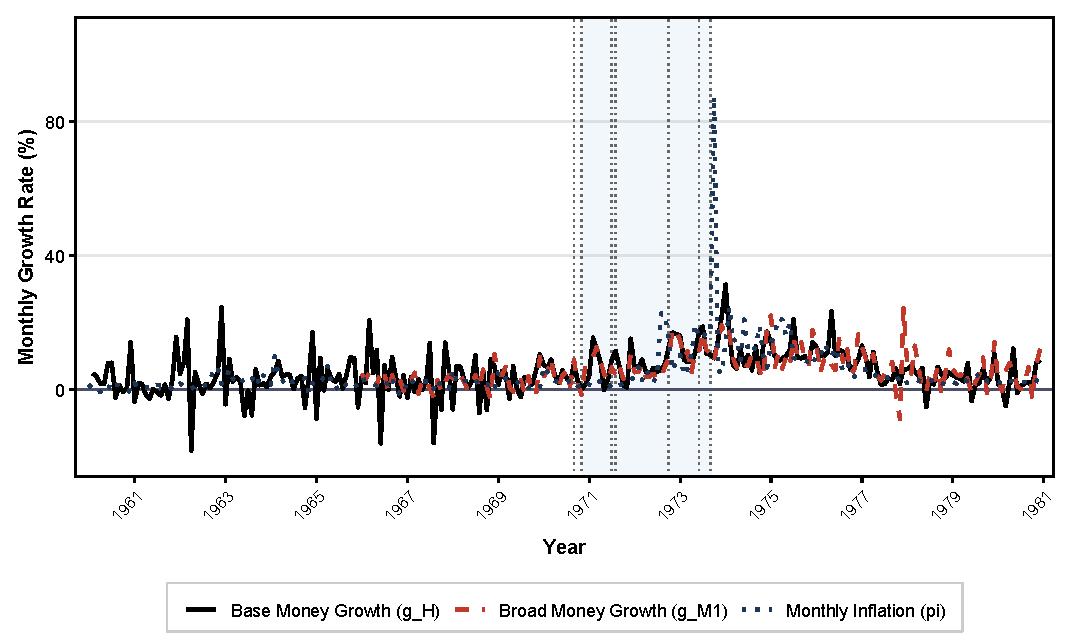
\includegraphics[width=0.88\textwidth]{figures/fig01d_money_growth_inflation.pdf}
\begin{minipage}{0.95\textwidth}
\vspace{0.2cm}
\footnotesize
\textbf{Notes:} Monthly series of base money growth ($g_{H,t}$, solid black line), broad money supply growth ($g_{M1,t}$, dashed red line), and monthly consumer price inflation ($\pi_t$, dotted blue line). Benchmark markers $\mathrm{I}$--$\mathrm{VII}$ defined in Table~\ref{tab:critical_junctures}. Shaded blue region designates the Unidad Popular government (1970--1973). Sourced from Banco Central de Chile REST API and Instituto Nacional de Estad\'{\i}sticas (INE).
\end{minipage}
\end{figure}

\begin{figure}[!htbp]
\centering
\caption{Observed Empirical Money Multiplier ($M1/H$, 1965--1980)}
\label{fig:money_multiplier}
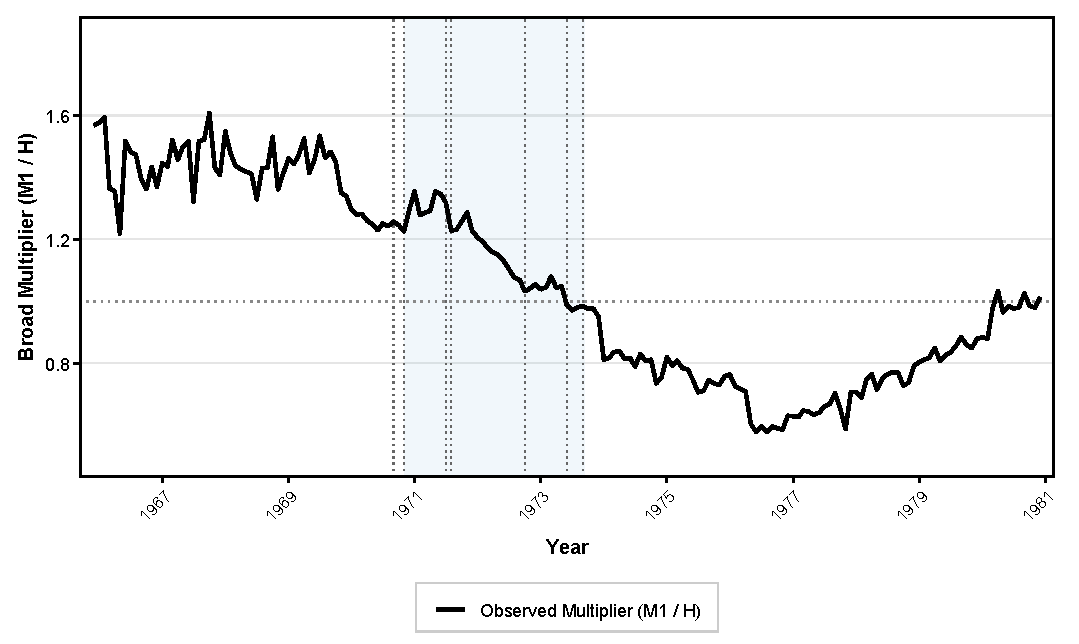
\includegraphics[width=0.88\textwidth]{figures/fig01e_money_multiplier.pdf}
\begin{minipage}{0.95\textwidth}
\vspace{0.2cm}
\footnotesize
\textbf{Notes:} Monthly trajectory of the broad-to-base money multiplier ($m_t \equiv M1_t / H_t$, solid black line). The figure is restricted to the observed M1 sample, December 1965--December 1980. Benchmark markers $\mathrm{I}$--$\mathrm{VII}$ defined in Table~\ref{tab:critical_junctures}. Shaded blue region designates the Unidad Popular government (1970--1973). Sourced from Banco Central de Chile REST API.
\end{minipage}
\end{figure}

In Figure~\ref{fig:money_growth_inflation}, base money ($g_H$) and broad money ($g_{M1}$) grew at monthly rates of $10\%\text{--}15\%$ through 1971 and early 1972, while physical manufacturing output expanded and wages rose. Monthly consumer inflation remained below $5\%$ during this initial phase, rising to $15.2\%$ in October 1972 as transport disruptions and commercial withholding emerged during the nationwide trucking strike. Central bank credit expansion accompanied rising enterprise operating costs and payroll requirements in subsequent months. The monthly peak of consumer inflation occurred in October 1973 ($+87.6\%$) following the military junta's Decree Law 522 price deregulation. This descriptive sequence is consistent with credit accommodation of cost pressures; Section~\ref{sec:granger_tournament} tests whether that directional relationship holds systematically.

Figure~\ref{fig:money_multiplier} tracks the empirical broad-to-base money multiplier ($m_t \equiv M1_t / H_t$). Under Frei (1966--1970), the multiplier fluctuated between $1.35$ and $1.60$. Under the UP administration, the ratio trended downward from $1.35$ in January 1971 to $0.98$ in August 1973, reaching a low of $0.58$ in 1976. Accelerating inflation co-moves visually with this compression in the broad-to-base ratio. Possible institutional mechanisms underlying this decline---including cash hoarding during shortages and central bank credit to socialized firms---are discussed in Sections~\ref{sec:macro_framework} and \ref{sec:discussion_conclusion}; Section~\ref{sec:granger_tournament} evaluates its predictive precedence relative to inflation.

\subsubsection{Real Production Divergence and Focused Monthly Windows}
\label{sec:stylized_real_production}

Figure~\ref{fig:manufacturing_mining} plots physical output dynamics across 1960--1980, documenting divergent paths between domestic manufacturing and export mining.

\begin{figure}[!htbp]
\centering
\caption{Real Physical Output Trajectories: Manufacturing vs. Mining (1960--1980)}
\label{fig:manufacturing_mining}
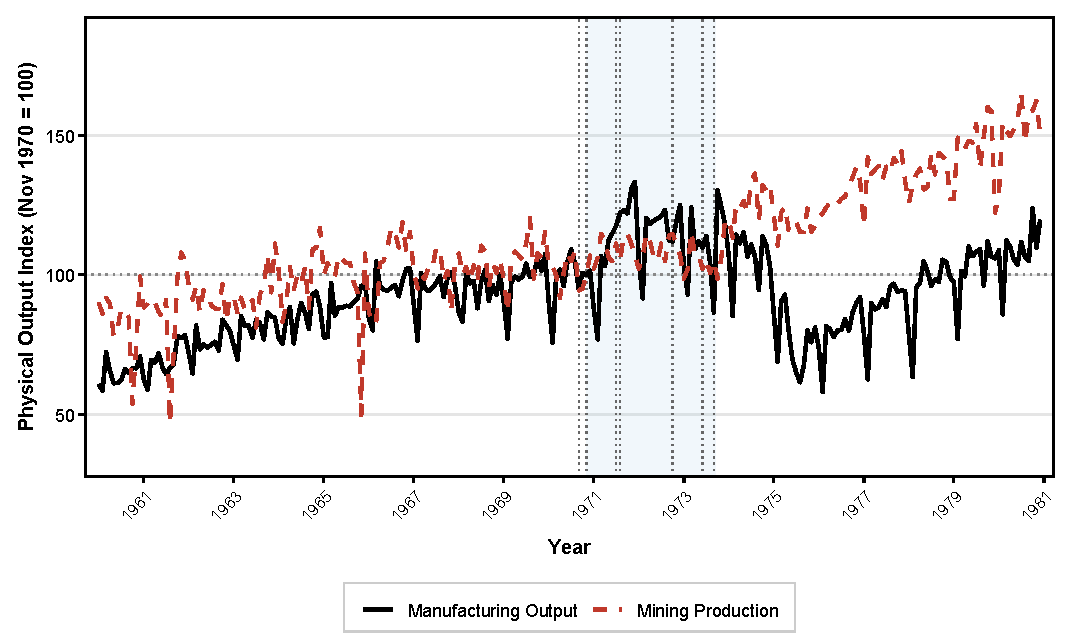
\includegraphics[width=0.88\textwidth]{figures/fig01c_manufacturing_mining.pdf}
\begin{minipage}{0.95\textwidth}
\vspace{0.2cm}
\footnotesize
\textbf{Notes:} Monthly series of physical output indices for manufacturing (solid black line) and mining (dashed red line), re-based to November 1970 = 100. Benchmark markers $\mathrm{I}$--$\mathrm{VII}$ defined in Table~\ref{tab:critical_junctures}. Shaded blue region designates the Unidad Popular government (1970--1973). Sourced from \citet{DiazBahamonde2023} historical database, compiled from INE and SOFOFA for manufacturing, and SERNAGEOMIN, ODEPLAN, and CODELCO for mining.
\end{minipage}
\end{figure}

Manufacturing output expanded by $33.3\%$ between November 1970 and December 1971, reflecting utilization of capacity in wage-goods industries. In contrast, copper mining output rose by $7.0\%$, held back by technical constraints and equipment import delays \citep{DeVylder1976}. Following the October 1972 strike, manufacturing output contracted as transport disruptions and intermediate input shortages took effect. Following the September 1973 coup, manufacturing production declined persistently, falling below index 65 by 1975 (a $>35\%$ contraction from its 1971 peak) amid tariff reductions and demand compression.

Figure~\ref{fig:event_windows} examines monthly dynamics around two institutional turning points.

\begin{figure}[!htbp]
\centering
\begin{subfigure}[b]{0.85\textwidth}
    \centering
    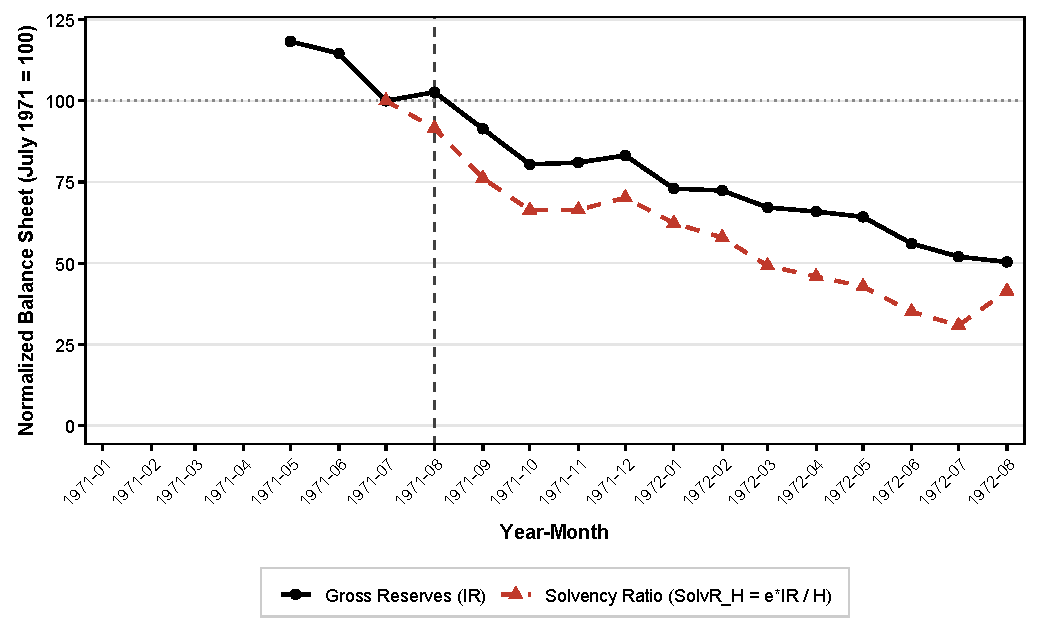
\includegraphics[width=\textwidth]{figures/fig02a_event_blockade_1971.pdf}
    \caption{August 1971 Credit Restrictions and Gold Suspension}
    \label{fig:event_blockade_1971}
\end{subfigure}
\vspace{0.3cm}

\begin{subfigure}[b]{0.85\textwidth}
    \centering
    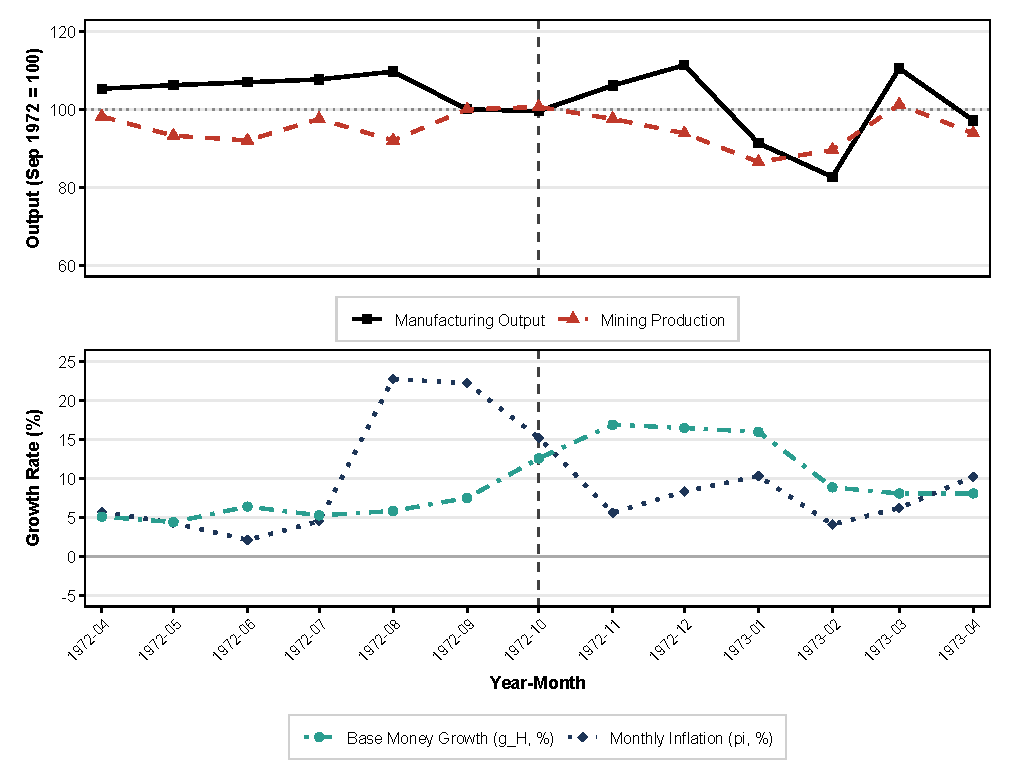
\includegraphics[width=\textwidth]{figures/fig02b_event_lockout_1972.pdf}
    \caption{October 1972 Lockout and Trucking Strike}
    \label{fig:event_lockout_1972}
\end{subfigure}
\caption{Monthly Trajectories around External and Supply Shocks (Chile, 1971--1972)}
\label{fig:event_windows}
\vspace{0.2cm}
\begin{minipage}{0.95\textwidth}
\footnotesize
\textbf{Notes:} Monthly series centered at $t=0$ around two institutional turning points. Panel~(a) tracks Central Bank Gross International Reserves ($IR_t$, solid black line with circle markers) and the Solvency Ratio relative to Base Money ($\text{SolvR}^{H}_t \equiv \frac{e_t \cdot IR_t}{H_t \cdot 1000}$, dashed red line with triangle markers), indexed to July 1971 = 100, around the August 1971 Eximbank credit denial and Bretton Woods gold-window suspension (Benchmark $\mathrm{IV}$). Panel~(b) aligns two vertical subpanels around the October 1972 Lockout (Benchmark $\mathrm{V}$): the upper panel displays physical output indices for Manufacturing (solid black line with square markers) and Mining Production (dashed red line with triangle markers), indexed to September 1972 = 100; the lower panel displays monthly consumer inflation ($\pi_t$, dotted dark-blue line with diamond markers) and Central Bank base money growth ($g_H$, dot-dashed teal line with circle markers) in genuine monthly growth percentages ($\%$) along a common horizontal time axis. Sourced from Banco Central de Chile REST API, IMF International Financial Statistics, and \citet{DiazBahamonde2023}.
\end{minipage}
\end{figure}

The first window centers on the August 1971 credit restrictions and suspension of dollar-gold convertibility (Figure~\ref{fig:event_blockade_1971}, $t=0$). Following the constitutional copper nationalization of July 11, the U.S. Export-Import Bank denied credit on August 12, and President Nixon suspended dollar-gold convertibility on August 15 \citep{Zoeller2019}. This monthly window illustrates the trajectory of reserve drain: gross international reserves fell from index $100.0$ to below $30.0$, and the Central Bank Solvency Ratio ($\text{SolvR}^{H}_t$) declined by more than $70\%$ over the subsequent twelve months. Reserve coverage had deteriorated substantially before the later acceleration in domestic money growth.

The second window centers on the October 1972 trucking strike and commercial lockout (Figure~\ref{fig:event_lockout_1972}, $t=0$). Transport paralysis and merchant shutdowns coincided with a 12 percentage-point drop in manufacturing output, while mining output in northern enclaves remained less affected. Monthly consumer inflation rose from $2.8\%$ to $15.2\%$. Base-money growth did not accelerate contemporaneously with the October jump in inflation; its acceleration followed at $t = +1$ and $t = +2$. The descriptive window places the price increase before the subsequent expansion in base-money growth. While this ordering is consistent with accommodation of cost pressures, establishing directional precedence requires the econometric testing developed below.

\subsubsection{Descriptive Synthesis and Empirical Transition}
\label{sec:stylized_synthesis}

Table~\ref{tab:marglin_monthly_grounding} presents macroeconomic indicators across six selected dates, and Table~\ref{tab:critical_junctures} summarizes the seven institutional events ($\mathrm{I}$--$\mathrm{VII}$).

\begin{table}[H]
\centering
\small
\caption{Monthly Macroeconomic Dynamics, Central Bank Solvency, and External Constraints across Structural Junctures (Chile, 1970--1973)}
\label{tab:marglin_monthly_grounding}
\label{tab:marglin_grounding}
\renewcommand{\arraystretch}{1.10}
\setlength{\tabcolsep}{4.8pt}
\resizebox{\textwidth}{!}{%
\begin{tabular}{lcccccc}
\toprule
& \textbf{Nov 1970} & \textbf{Aug 1971} & \textbf{Dec 1971} & \textbf{Oct 1972} & \textbf{Aug 1973} & \textbf{Dec 1973} \\
\textbf{Macroeconomic Variable} & \textit{Inauguration} & \textit{Gold Suspension} & \textit{Output Peak} & \textit{October Lockout} & \textit{Pre-Coup} & \textit{Post-Coup} \\
\midrule
\multicolumn{7}{l}{\textbf{A. Inflation and Price Dynamics}} \\[0.2em]
Monthly Inflation (\%) & 0.6\% & 1.1\% & 2.8\% & 15.2\% & 17.1\% & 4.7\% \\
YoY Inflation (\%) & 35.3\% & 17.4\% & 22.1\% & 142.9\% & 303.6\% & 508.1\% \\
\midrule
\multicolumn{7}{l}{\textbf{B. Real Physical Activity (Nov 1970 = 100)}} \\[0.2em]
Manufacturing Output Index & 100.0 & 122.0 & 133.3 & 111.9 & 104.6 & 118.1 \\
Mining Production Index & 100.0 & 104.9 & 107.0 & 114.7 & 100.7 & 119.6 \\
\midrule
\multicolumn{7}{l}{\textbf{C. Central Bank Solvency and Monetary Backing}} \\[0.2em]
Gross International Reserves (USD M) & 408.0 & 268.1 & 217.2 & 103.4 & 114.2 & 179.7 \\
Solvency Ratio Base ($\text{SolvR}^H \equiv \frac{e \cdot IR}{H \cdot 1000}$) & 0.63 & 0.22 & 0.17 & 0.07 & 0.06 & 0.25 \\
Solvency Ratio M1 ($\text{SolvR}^{M1} \equiv \frac{e \cdot IR}{M1 \cdot 1000}$) & 0.51 & 0.18 & 0.14 & 0.07 & 0.06 & 0.27 \\
Observed Multiplier ($M1/H$) & 1.23 & 1.23 & 1.23 & 1.03 & 0.98 & 0.95 \\
Base Money Monthly Growth ($g_H$) & 0.0\% & 11.5\% & 15.1\% & 12.6\% & 10.7\% & 21.8\% \\
M1 Money Monthly Growth ($g_{M1}$) & -1.6\% & 4.3\% & 10.2\% & 9.1\% & 11.6\% & 19.2\% \\
\midrule
\multicolumn{7}{l}{\textbf{D. Official Exchange Rate and World Commodity Prices}} \\[0.2em]
Official Exchange Rate ($e_t$) & 0.012 & 0.0122 & 0.0146 & 0.0250 & 0.0740 & 0.34 \\
World Copper Price (USD/lb) & \$0.492 & \$0.499 & \$0.471 & \$0.466 & \$0.948 & \$1.011 \\
World Gold Price (USD/oz) & \$37.44 & \$42.71 & \$43.48 & \$64.86 & \$106.76 & \$106.72 \\
\midrule
\multicolumn{7}{l}{\textbf{E. External Trade, Capacity to Import, and Structural Imbalance}} \\[0.2em]
Export Activity Index & 2.68 & 1.71 & 1.73 & 1.46 & 2.31 & 2.81 \\
Import Activity Index & 1.51 & 3.54 & 3.11 & 1.79 & 4.11 & 2.86 \\
Real Trade Ratio ($\text{Exp}/\text{Imp}$) & 1.78 & 0.48 & 0.56 & 0.82 & 0.56 & 0.98 \\
Real Capacity to Import ($M^{\text{cap}}_t$, Nov 1970 = 100) & 100.0 & 62.5 & 59.5 & 47.7 & 129.5 & 168.7 \\
Effective Real Imports ($M_t$, Nov 1970 = 100) & 100.0 & 234.5 & 206.2 & 118.4 & 272.3 & 189.4 \\
Real Structural Imbalance ($\Theta_t$, \%) & 100.0\% & 374.9\% & 346.4\% & 248.1\% & 210.3\% & 112.3\% \\
US Wholesale Price Index (Nov 1970 = 100) & 100.0 & 103.8 & 104.0 & 108.1 & 128.0 & 127.8 \\
\bottomrule
\end{tabular}%
}
\vspace{0.3em}
\begin{minipage}{\textwidth}
\footnotesize \textbf{Sources and Notes:} Primary monthly series from Central Bank of Chile and IMF International Financial Statistics. Gross international reserves ($IR_t$) represent official foreign exchange holdings from IMF IFS. Solvency Ratio defined relative to Base Money as $\text{SolvR}^{H}_t \equiv (e_t \cdot IR_t) / (H_t \cdot 1000)$ and relative to M1 as $\text{SolvR}^{M1}_t \equiv (e_t \cdot IR_t) / (M1_t \cdot 1000)$, where $IR_t$ is in USD millions, $e_t$ is the official exchange rate in pesos per USD (standardized per BCCh historical conventions), and $H_t, M1_t$ are recorded in thousands of millions of pesos (billions, \emph{miles de millones de pesos}), scaled by $1{,}000$ to express monetary liabilities in millions of pesos and ensure dimensional consistency with the numerator ($e_t \cdot IR_t$). Capacity to Import Index operationalizes the Prebisch-ECLAC formula: $M^{\text{cap}}_t \equiv (\text{Exports}_t / \text{Exports}_{70:11}) \times [(P^{\text{Cu}}_t / P^{\text{Cu}}_{70:11}) / (P^{\text{US}}_{W,t} / P^{\text{US}}_{W,70:11})] \times 100$. Real Structural Imbalance Ratio defined as $\Theta_t \equiv (M_t / M^{\text{cap}}_t) \times 100$, tracking the physical quantum of imports relative to real export purchasing power. Selected dates mark historical milestones: Nov 1970 (Allende inauguration baseline); Aug 1971 (Eximbank credit denial and suspension of dollar-gold convertibility); Dec 1971 (cyclical output peak); Oct 1972 (national trucking strike and commercial lockout); Aug 1973 (late administration baseline before the September coup); and Dec 1973 (post-coup benchmark following October 1973 Decree Law 522 price deregulation).
\end{minipage}
\end{table}


\begin{table}[H]
\centering
\small
\caption{Chronology of Critical Macroeconomic Junctures and Institutional Shocks (Chile, 1970--1973)}
\label{tab:critical_junctures}
\renewcommand{\arraystretch}{1.15}
\resizebox{\textwidth}{!}{%
\begin{tabular}{clllp{6.8cm}}
\toprule
\textbf{Ref} & \textbf{Date} & \textbf{Historical Juncture} & \textbf{Institutional Shock Mechanism} & \textbf{Macroeconomic / Balance-Sheet Transmission Channel} \\
\midrule
$\mathrm{I}$   & Sep 1970 & Presidential Election & Electoral panic; commercial deposit runs & Capital flight ($EO < 0$); foreign currency accumulation; Central Bank emergency rediscounts. \\
$\mathrm{II}$  & Nov 1970 & Inauguration Baseline & Allende assumes presidency; tariff and price freeze & Initial price stabilization; real wage gains; inherited gross reserve buffer (\$408.0M; $\text{SolvR}^H = 0.63$; $\text{SolvR}^{M1} = 0.51$). \\
$\mathrm{III}$ & Jul 1971 & Copper Nationalization & Unanimous constitutional reform (Law 17,450) & Sovereign recovery of \textit{Gran Miner\'ia}; triggers bilateral U.S. credit restrictions and legal liens. \\
$\mathrm{IV}$  & Aug 1971 & Eximbank Embargo \& Bretton Woods Collapse & U.S. credit freeze; dollar-gold convertibility suspended & Revolving trade credits reduced (\$220M $\to$ \$35M); cash-in-advance imports; reserve drain accelerates ($\Delta IR = -\$140$M). \\
$\mathrm{V}$   & Oct 1972 & October Lockout (\textit{Paro de Octubre}) & Trucking strike; SOFOFA commercial lockout & Physical transport paralysis; wholesale inventory withholding; monthly inflation rises to $15.2\%$; central bank liquidity accommodation. \\
$\mathrm{VI}$  & Jun 1973 & \textit{El Tanquetazo} & Military uprising (2nd Armored Regiment) & Heightened political instability; logistical disruption; black market expansion; reserve depletion and structural trade imbalance ($\Theta_t = 210.3\%$). \\
$\mathrm{VII}$ & Sep 1973 & Military Coup d'\'Etat & Violent overthrow; followed by October DL 522 deregulation & Elimination of price controls; $+87.6\%$ MoM inflation jump in October; real wage contraction ($-40\%$); domestic expenditure compression. \\
\bottomrule
\end{tabular}%
}
\begin{tabular}{p{0.95\textwidth}}
\footnotesize \textbf{Notes:} Master reference chronology for vertical benchmark lines appearing across high-frequency time series (Figures~\ref{fig:solvency_reserves}--\ref{fig:money_multiplier}) and defining intervention cutoffs for focused monthly windows (Figures~\ref{fig:event_blockade_1971}--\ref{fig:event_lockout_1972}) and companion econometric estimation stages.
\end{tabular}
\end{table}


Table~\ref{tab:marglin_monthly_grounding} illustrates this temporal sequence across the selected dates: between November 1970 and August 1971---while monthly consumer inflation remained low ($1.1\%$) and industrial manufacturing output was expanding ($+22.0\%$)---the Central Bank Solvency Ratio ($\text{SolvR}^{H}_t$) had declined from $0.63$ to $0.22$, and gross foreign reserves had fallen by $\$139.9$ million. External balance-of-payments deterioration preceded the subsequent acceleration of domestic inflation and credit expansion.

Across the selected dates, reserve coverage deteriorated substantially before the sharp acceleration of inflation in late 1972. Money growth, inflation, exchange-rate adjustment, and trade imbalances moved together during much of the crisis, so these descriptive sequences do not establish their direction of dependence. Section~\ref{sec:granger_tournament} evaluates directional predictive precedence through Granger-causality tests in stationary vector autoregressions across six modular empirical systems. Section~\ref{sec:tvar_solvency_regimes} then estimates a non-linear Threshold Vector Autoregression (TVAR) conditioned on the monthly Solvency Growth Gap ($\Delta s_{t-1} \equiv g^F_{t-1} - g^H_{t-1}$) to test whether these relationships change under conditions of central bank insolvency.
